\documentclass[11pt]{article}

\usepackage[utf8]{inputenc}
\usepackage[T1]{fontenc}
\usepackage[francais]{babel}
\usepackage[top=1.8cm, bottom=1.8cm, left=1.8cm, right=1.8cm]{geometry}
\usepackage{hyperref}
\usepackage{graphicx}
\usepackage{epsfig}
\usepackage{array}
\hypersetup{
    colorlinks=true,
    breaklinks=true,
    urlcolor=red,
}
\parskip=5pt

\title{Cahier des charges}
\author{Pierre AYOUB, Claire BASKEVITCH, Tristan BESSAC, \\
Clément CAUMES, Damien DELAUNAY, Yassin DOUDOUH}
\date{Mercredi 14 Mars 2018}

\begin{document}

\title{\Huge{\textbf{Cahier Des Charges}}}
	\author{AYOUB Pierre - BASKEVITCH Claire - BESSAC Tristan - \\
		CAUMES Clément - DELAUNAY Damien - DOUDOUH Yassin \\ \\ \\
		Stéganographie \& Stéganalyse \\ \\ \\}
		

	\begin{titlepage}
		\maketitle
		\vspace{20em}
		\begin{center}
\includegraphics{application.png}\end{center}
	\end{titlepage}

\section{Préambule}

\subsection{Définition des termes du sujet}
La stéganographie est l'art de la dissimulation, appliquée en informatique en
cachant des données dans d'autres données. Cette dissimulation se fait
généralement au sein de fichiers multimédias. 
La stéganographie se différencie de la cryptographie, qui correspond à chiffrer un message afin qu'il soit illisible par une personne différente de l'émetteur 
et du destinataire. 
En effet, un message chiffré en cryptographie sera visible par tous mais illisible, tandis qu'un message caché dans un fichier $f$ en stéganographie ne sera vu que si un inconnu sait que $f$ contient un message et connaît l'algorithme pour l'interpréter. 

La stéganalyse, quant à elle, est la recherche de données cachées dans des fichiers suspects. Si ces données sont identifiées, il faut ensuite réussir à les
extraire pour les lire. Il s'agit donc de la méthode inverse à la stéganographie. 

\subsection{Historique}
La stéganographie est une méthode très ancienne dont la première référence à cette utilisation date du premier siècle avant Jésus-Christ. 
Elle apparaît dans un récit écrit par Hérodote qui raconte comment deux citoyens communiquaient secrètement : 
le premier citoyen rasait la tête de son esclave et lui écrivait un message sur son crâne. Ensuite, il fallait attendre que les cheveux de l'esclave repoussent puis envoyer ce dernier chez le deuxième citoyen. 
Ce citoyen devait de nouveau raser la tête de l'esclave pour découvrir le message qui lui était destiné. 
Une autre utilisation de la stéganographie consistait à utiliser de l'encre, invisible à l'oeil nu, mais qui était révélée à la chaleur. 

Avec l'émergence de l'informatique, les techniques de stéganographie se sont renouvelées. En effet, il est désormais possible de cacher des données dans d'autres données. 
Cette multiplicité de techniques stéganographiques, grâce à l'informatique, montre l'étendue de cette application dans tous les domaines. 
Par exemple, la stéganographie moderne a été utilisée dans des communications terroristes (transmission de messages) ou dans les signatures de fichiers multimedia (tatouage numérique) afin de protéger les droits d'auteurs. 

\section{Conducteurs du projet}

\subsection{But du projet}
Le but du projet est de réaliser un logiciel de stéganographie permettant à des personnes lambdas de communiquer sans que l'on soupçonne que leurs communications soient en réalité compromettantes. 

Le but de l'application est de permettre à un utilisateur $U_1$ d'envoyer des données cachées à un autre utilisateur $U_2$. Ce deuxième utilisateur devra pouvoir interpréter ces données en utilisant la même application que $U_1$. 

\subsection{Motivation du projet}

La motivation du projet est venue par notre envie de la majorité des membres de ce groupe de projet d'obtenir le master SeCReTs. 
En effet, nous voulions tous réaliser un projet en rapport à la cryptographie et c'est donc pour cela que nous nous sommes réunis afin de réaliser ce type de projet. 

\section{Contraintes du projet}

\subsection{Calendrier}

Le Calendrier est imposé et suit les étapes suivantes : 

\begin {itemize}
\item Le Cahier des Charges doit être remis le 14 mars. 
\item Le Cahier des Spécifications est à remettre le 18 avril. 
\item La remise du produit au client est le 25 mai. 
\item La présentation du produit au client sera le 1 juin 2018.  
\end{itemize}


\subsection{Contraintes imposées}
Plusieurs contraintes sont imposées par le client : 
\begin{itemize}
\item le produit permettra à celui qui l'utilise de cacher des données dans des fichiers de différents types : les types Image, Audio et Video seront pris en charge. Les formats seront choisis par le concepteur de l'application. 
\item le fichier à analyser sera déjà considéré comme hôte : on sait à l'avance que celui-ci contient des données à extraire et il faut donc les prélever. 
\item l'application aura une interface graphique : elle sera manipulée par les utilisateurs voulant découvrir un message envoyé par quelqu'un (ayant utilisé cette même application), ou voulant cacher des données dans un fichier. 
Il devra néanmoins choisir un fichier hôte que l'application puisse manipuler. 
\item le logiciel proposera également une interface en ligne de commande : elle proposera les mêmes fonctionnalités que l'interface graphique. 
\end{itemize}

\section{Exigences fonctionnelles}
\subsection{Portée du produit}
L'application sera utilisée par des utilisateurs qui pourront tous faire les mêmes actions : dissimuler des données dans un fichier image, son et vidéo (partie stéganographie). 
Il pourra également savoir si un fichier contient des données cachées et les extraire (stéganalyse). 
Cela permettra à un utilisateur d'insérer des données cachées dans un fichier, afin de l'envoyer à un autre utilisateur. Ce dernier va ensuite faire la tâche inverse : extraire ces données cachées. 

\subsection{Exigences du client}
L'application doit respectée deux exigences pour le client : elle doit permettre à un utilisateur ne connaissant pas la stéganographie de pouvoir facilement utiliser toutes les fonctionnalités de 
l'application grâce à une interface graphique. De plus, une interface au terminal doit être également proposée pour les utilisateurs savant manipuler le terminal. En effet, ces utilisateurs pourront réaliser les mêmes fonctionnalités qu'avec l'interface graphique. 

\section{Exigences non fonctionnelles}
\subsection{Apparence et Perception}
Le logiciel doit permettre à n'importe quel utilisateur de pouvoir cacher ses données dans des fichiers. En effet, la facilité d'utilisation de l'application sera ciblée pour le développement. 
Il sera facile de naviguer entre les deux menus : si l'utilisateur veut cacher ses données ou s'il veut découvrir les données cachées dans un fichier. 
Il pourra naviguer dans son système de gestion de fichiers afin de choisir quelles données cachées et quel fichier contiendra ces données cachées. 

\subsection{Performance}
L'application devra être rapide pour l'utilisateur qui s'en sert. Bien entendu, la stéganographie sur certains fichiers lourds (tels que des fichiers de type video) rendra l'exécution plus lente 
mais elle ne devra pas être trop importante pour l'utilisateur. 

\subsection{Exigences culturelles, politiques et légales}
L'application de stéganographie vise des clients en France. Il faut donc respecter les lois françaises concernant l'utilisation de cette application. 
La loi du 21 juin 2004, pour la confiance dans l'économie numérique, définit cette application comme moyen de cryptologie car elle vise à transformer des données pour garantir la sécurité de la transmission de celles-ci. 
Par ailleurs, l'article 30 de cette même loi oblige la déclaration de l'application si cette dernière est importée et/ou exportée. 

\newpage

\section{Modules du produit}

\subsection{Organigramme}

\hspace{1cm}
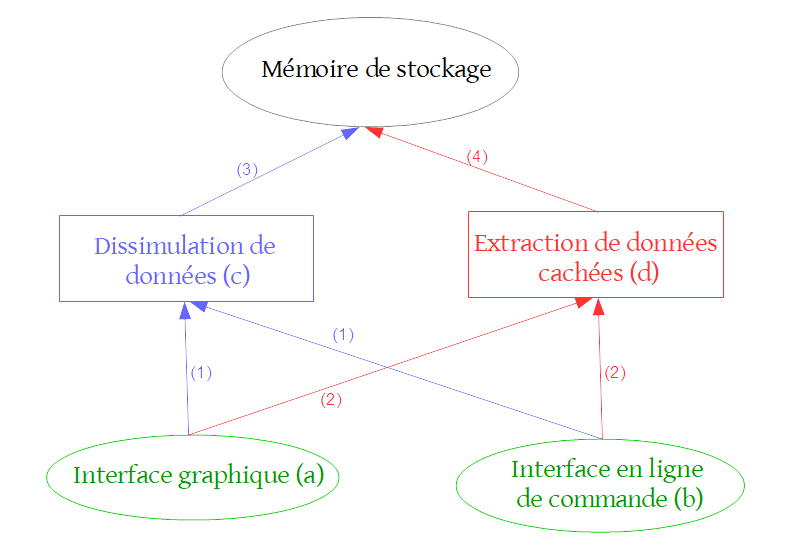
\includegraphics[scale=0.55]{organigramme.png}

\paragraph{Liste des modules et de leurs fonctionnalités}
\begin{description}
\item[a)] \textbf{Interface graphique / Interface en ligne de commande} : interfaces permettant à l'utilisateur de choisir parmi les deux fonctionnalités possibles de l'application. 
Il peut dissimuler des données dans un fichier (dont le type et le format sont pris en charge par l'application). Ou bien, il peut extraire les données cachées dans un fichier. 

\item[b)] \textbf{Compatibilité} : le format du fichier hôte (pour le module \textit{Dissimulation de données}) ou le format du fichier à analyser (pour le module \textit{Extraction de données cachées}), 
choisis par l'utilisateur, sont vérifiés pour savoir s'il est bien pris en charge par l'application. 

\item[c)] \textbf{Proposition des algorithmes de stéganographie} : en fonction du type et du format du fichier hôte, ainsi que de la taille des données à cacher, 
un ou plusieurs algorithmes seront proposés. 

\item[d)] \textbf{Détection de l'algorithme de stéganographie} : analyse du fichier pour découvrir quel algorithme a été utilisé afin de les extraire correctement par la suite. 

\item[e)] \textbf{Insertion des données} : la copie des données du fichier hôte sera modifiée avec l'insertion des données à cacher à l'aide de l'algorithme choisi par l'utilisateur. 

\item[f)] \textbf{Extraction} : les données cachées dans le fichier à analyser sont extraites. 

\end{description}

\paragraph{Liste des informations qui circulent entre les modules}

\small
\begin{description}
\item[1)] 
\begin{itemize}
\item utilisation de l'application (dissimulation ou extraction)
\item nom du fichier hôte, nom du fichier à cacher et chemin du fichier à créer (pour la dissimulation)
\item nom du fichier à analyser et chemin du fichier résultant de l'extraction des données cachées (pour l'extraction)
\end{itemize}
\item[2)] 
\begin{itemize}
\item nom du fichier hôte 
\item nom du fichier à cacher 
\item chemin du fichier à créer, qui dissimulera les données à cacher et ayant l'apparence de l'hôte
\end{itemize}
\item[3)] 
\begin{itemize}
\item nom du fichier contenant les données cachées à analyser
\item chemin du fichier résultant de l'extraction des données cachées
\end{itemize}
\item[4)] 
\begin{itemize}
\item nom du fichier hôte et nom du fichier à cacher (pour la dissimulation)
\item nom du fichier contenant les données cachées à analyser (pour l'extraction)
\end{itemize}
\item[5)]
\begin{itemize}
\item fichier hôte et fichier à cacher (pour la dissimulation)
\item fichier contenant les données cachées à analyser (pour l'extraction)
\end{itemize}
\item[6)]
\begin{itemize}
\item fichier hôte 
\item fichier à cacher 
\item chemin du fichier à créer, qui dissimulera les données à cacher
\end{itemize}
\item[7)]
\begin{itemize}
\item fichier contenant les données cachées à analyser
\item chemin du fichier résultant de l'extraction des données cachées
\end{itemize}
\item[8)]
\begin{itemize}
\item liste des algorithmes que l'utilisateur peut utiliser (selon le format du fichier hôte et la taille des données à cacher)
\end{itemize}
\item[9)]
\begin{itemize}
\item choix de l'algorithme par l'utilisateur
\item mot de passe choisi par l'utilisateur (s'il a sélectionné la méthode cryptographique parmi les algorithmes de stéganographie)
\end{itemize}
\item[10)]
\begin{itemize}
\item choix de l'algorithme détecté dans le fichier à analyser
\end{itemize}
\item[11)]
\begin{itemize}
\item mot de passe pour déchiffrer les données à extraire (si l'algorithme de stéganographie utilise la méthode cryptographique)
\end{itemize}
\item[12)]
\begin{itemize}
\item fichier hôte
\item fichier à cacher
\item chemin du fichier à créer lors de la dissimulation de données
\item nom de l'algorithme de stéganographie utilisé
\end{itemize}
\item[13)]
\begin{itemize}
\item fichier contenant les données cachées à analyser 
\item chemin du fichier résultant de l'extraction des données cachées
\item nom de l'algorithme détecté
\end{itemize}
\item[14)]
\begin{itemize}
\item données de l'hôte où les données à cacher ont été insérées en utilisant l'algorithme de stéganographie
\end{itemize}
\item[15)]
\begin{itemize}
\item données cachées extraites du fichier à analyser
\end{itemize}
\end{description}

\normalsize
\subsection{Algorithmes des fonctionnalités}
L'application permettra de cacher des données dans des fichiers de différents formats (image, son, video). 
Plusieurs méthodes seront utilisées : 

\subsubsection{Algorithme LSB (Least Significant Bit)}
L'algorithme LSB permet de cacher des bits dans des octets tel qu'ils seront invisibles pour l'Homme. 
Il permet de cacher des données dans un fichier sans en altérer sa taille. 
Dans le cas de la stéganographie sur image, chaque pixel d'une image correspond à un triplet de nombres : R,G,B qui correspondent aux composantes de couleurs Rouge-Vert-Bleu de 0 à 255. 
Le but de cet algorithme est donc de cacher des bits dans cette image. Pour se faire, nous allons remplacer les 2 bits de poids faibles de chaque composante des pixels de l'image. 
En effet, à l'oeil nu, l'homme ne discernera jamais le changement minime de composante. 
Prenons un exemple de couleur $C_1$ dont le triplet est $(219,27,91)$. 

R : $219_{10} = 11011011_2$	\qquad G : $27_{10} = 11011_2$ \qquad B : $91_{10} = 1011011_2$


Imaginons que la donnée à cacher dans le fichier composé de cet unique pixel de couleur $C_1$ correspond à la suite de bits $B = 000000_2$.
Ce qui donne une toute autre couleur $C_2$ en changeant les 2 bits de poids faibles de chaque composantes du pixel : 

R : $216_{10} = 11011000_2$ \qquad G : $24_{10} = 11000_2$ \qquad B : $88_{10} = 1011000_2$


Voici ici les deux couleurs $C_1$ et $C_2$, montrant ainsi qu'un humain ne pourra jamais détecter un changement de bit : 

\begin{figure}[h]
 \begin{minipage}{.46\linewidth}
  \centering\epsfig{figure=219_27_91.png}
  \caption{Couleur $C_1$}
 \end{minipage} \hfill
 \begin{minipage}{.46\linewidth}
  \centering\epsfig{figure=216_24_88.png}
  \caption{Couleur $C_2$}
 \end{minipage}
\end{figure}

Cet algorithme peut également s'appliquer à d'autres types de fichiers : pour le son, il est possible de modifier très peu les fréquences sonores sans en altérer le bruit ; 
pour la video, un fichier video est composé de frames (images de la vidéo) et il est donc possible de manipuler les données pour pouvoir en cacher d'autres. 

Pour la partie réception du fichier, il faut savoir si ce fichier a été utilisé pour un message caché et connaître combien de bits sont cachés. 
Il faudra donc calculer la taille maximale du message à cacher qui sera une puissance de 2. En effet, en fonction de la taille du fichier, un certain nombre de bits sera réservé pour connaître la taille 
des données à cacher. 
En fonction de ces informations, la suite de bits cachée sera donc formée.

\subsubsection{Algorithme EOF (End Of File)}
Chaque format de fichier a une mise en forme unique permettant de décrire facilement n'importe quelles données. 
L'entête du fichier va contenir sa signature (Magic Number) ainsi que plusieurs octets décrivant ce fichier, puis, le réel contenu du fichier, visible par l'utilisateur grâce à un éditeur. 
Cet éditeur de fichiers va donc lire les données contenues dans le fichier en les interprétant. 

Pour que l'éditeur sache quand la lecture doit s'arrêter, le fichier va contenir, à la toute fin, un octet représentant la fin du fichier (EOF). 
Si des données existent après ce EOF, elles ne seront pas interprétées par l'éditeur. 
L'algorithme EOF est un algorithme très utilisé dans la stéganographie pour cacher des données : il consiste à écrire une suite de bits, représentant les données à cacher, dans le fichier où l'on va cacher ces dernières. 

\subsubsection{Méthode manipulant les Métadonnées}
Les fichiers multimédias, tels que les images, les sons et les vidéos, contiennent plusieurs types de données. 
Tout d'abord, la majeure partie du fichier représente les données du fichier en elles-mêmes. Dans le cas d'une image, on pourrait donner l'exemple des données représentant chaque pixel de l'image. 

De plus, souvent en amont du fichier, il existe des métadonnées, servant à décrire le fichier représenté. Par exemple, pour une image, il est utile de stocker la taille en pixels de l'image afin que l'éditeur sache la représenter correctement. 
Il y a notamment des zones du fichier, réservées à l'utilisateur, afin qu'il mette des commentaires, par exemple pour représenter l'origine du fichier. 
Ces métadonnées ne sont pas interprétées directement par l'éditeur du fichier car la manipulation de celles-ci reste "complexe" pour un non-informaticien. 

De ce fait, les métadonnées sont très utilisées en stéganographie. Elles permettent d'insérer des données qui seront interprétées par le module de stéganalyse de l'application. 
Pour pouvoir cacher des données en manipulant les métadonnées, il faut donc analyser chaque format pris en charge par l'application, afin de connaître les détails des différents morceaux de données présents dans le fichier. 

\subsection{Estimations des coûts}
\begin{tabular}{|c|c|c|c|}
  \hline
  \textbf{Module} & \textbf{Coût en nombre} & \textbf{Coût en} & \textbf{Personnel(s) en charge} \\
   \textbf{de l'application} & \textbf{de lignes} & \textbf{temps} & \textbf{du module} \\
  \hline
  Stéganographie \& Stéganalyse & X & X & CAUMES Clément \&\\
   au format Image & lignes & heures & DOUDOUH Yassin\\
  \hline
  Stéganographie \& Stéganalyse & X & X & AYOUB Pierre \&\\
   au format Audio & lignes & heures & DELAUNAY Damien\\
  \hline
  Stéganographie \& Stéganalyse & X & X & BASKEVITCH Claire \&\\
   au format Video & lignes & heures & BESSAC Tristan\\
  \hline
  Interface en ligne de commande & X lignes & X heures & X\\ 
  \hline
  Interface graphique & X lignes & X heures & X\\
  \hline
\end{tabular}

\section{Autres aspects du projet}
\subsection{Solutions sur étagère déjà existantes}
Plusieurs applications de stéganographie existent déjà. En effet, elles peuvent cacher des données dans différents formats de fichiers image, audio et video. 
Pourtant, nous avons recensé 23 applications de stéganographie et seulement une seule propose de cacher des données dans des fichiers image, son et video. 
Tous les autres ne s'occupent que des images. 

\subsection{Tâches à réaliser pour le développement de l'application}
\begin {enumerate}
\item Identification du produit : étude des volontés et des demandes du client (énoncé du projet 24/01/18)
\item Etude du produit : recherche des outils et des algorithmes pour répondre au produit demandé par le client ; 
devis livré au client avec l'estimation des coûts du produit (cahier des charges 14/03/18)
\item Mise en relation avec le client : présentation du produit et de ses différents modules et fonctionnalités (présentation orale 21/03/18)
\item Etude spécifique du projet : identification précise des méthodes utilisées pour répondre aux demandes du client (spécifications 18/04/18)
\item Remise du produit au client : finalisation du produit et rendu de manuel d'utilisation et du compte-rendu (remise du compte rendu 25/05/18)
\item Démonstration du produit devant le client : explications fonctionnelles du produit (soutenance 01/06/18)
\end{enumerate}

\subsection{Améliorations pour les versions futures du projet}
La stéganographie se distingue de la cryptographie par le fait que, dans l'un, le message caché est visible par tous si celui-ci est extrait ; tandis que, dans l'autre, 
le message est transmis en étant chiffré sur un canal non-sûr. 

Pour une projection à long terme, dans d'éventuelles versions du logiciel, nous pourrions améliorer l'application en chiffrant les données cachées. 
En effet, lors de l'interception d'un éventuel fichier cachant des données, il faudra, en plus de les extraire, les déchiffrer : ce qui rend la tâche beaucoup plus longue
pour celui qui intercepte le fichier et qui tente de récupérer ces données cachées. 

De plus, pour la versatilité de l'application, nous pourrions prendre en charge de nouveaux formats (Image, Audio, Video). Cela permettrait d'augmenter la 
portée du logiciel. La manipulation de données compressées serait également une amélioration conséquente. 

L'ajout de nouveaux algorithmes de stéganographie permettrait de diminuer la détectabilité afin d'améliorer la sécurité de la stéganographie. 

\subsection{Choix du langage et de l'interface}

\section{Conclusion}
Après l'étude des demandes du client, nous mettrons en avant l'application StegX. Ainsi, ce logiciel aura deux modules : d'une part, il permettra de cacher des fichiers de toute sorte dans 
des fichiers de type Image, Audio et Video. D'autre part, il offrira la possibilité à ces utilisateurs d'analyser des fichiers (Image, Audio, Video) afin d'extraire les données cachées, s'ils en 
contiennent. 

Cette application sera implémentée par un groupe de six étudiants en Licence Informatique de l'Université de Versailles, ayant l'ambition d'obtenir un master en Cryptographie et Sécurité informatique (SeCReTs). 
Pour la gestion de projet, la méthode Gantt a été utilisée afin de réussir au mieux l'implémentation de cette application. 

\newpage
\section{Bibliographie}
\begin {itemize}
\item Compréhension de la méthode Volere pour la rédaction du cahier des charges : \url{http://www.qualitystreet.fr/2007/07/02/specifications-exigences-et-cahier-des-charges-comment/}
\end{itemize}

\end{document}

